\documentclass[12pt,twoside,a4paper,leqno,titlepage]{article}

\makeatletter
\newcommand{\ps@pagenumberfoot}{
\renewcommand{\@oddfoot}{\hfil\thepage}
   \renewcommand{\@evenfoot}{\thepage\hfil}
}
\makeatother

\input{Tyyli_utf.sty}
\pagestyle{pagenumberfoot}
\title{Dokumentaatio}
\author{Tomi Heiskanen}

\setlength{\parindent}{0pt}   
\setlength{\parskip}{1.6ex}
\setlength{\textwidth}{380pt}
\setlength{\evensidemargin}{40pt}
\setlength{\oddsidemargin}{40pt}

\begin{document}

\maketitle

\
\thispagestyle{empty}
\newpage

\setcounter{page}{1}
\tableofcontents
\thispagestyle{empty}

\newpage
\section{Johdanto}

Työn aiheena on kurssikysely. Kurssikyselyn avulla kerätään oppilaiden
mielipiteitä ja ideoita kurssin kehittämiseksi. Näiden avulla opettaja voi
kehittää omaa opetusta ja käytettäviä menetelmiä. Oppilaat voivat vastata
kyselyyn nimettömästi.

Työ toteutetaan Helsingin yliopiston tietojenkäsittelytieteen laitoksen users
palvelimella Apache-palvelimen alla. Web-sovelluksen alustajärjestelmän tulee
tukea php-kieltä ja PostgreSQL-tietokantaa.

\section{Yleiskuva järjestelmästä}

\begin{figure}[!h]
  \centering
  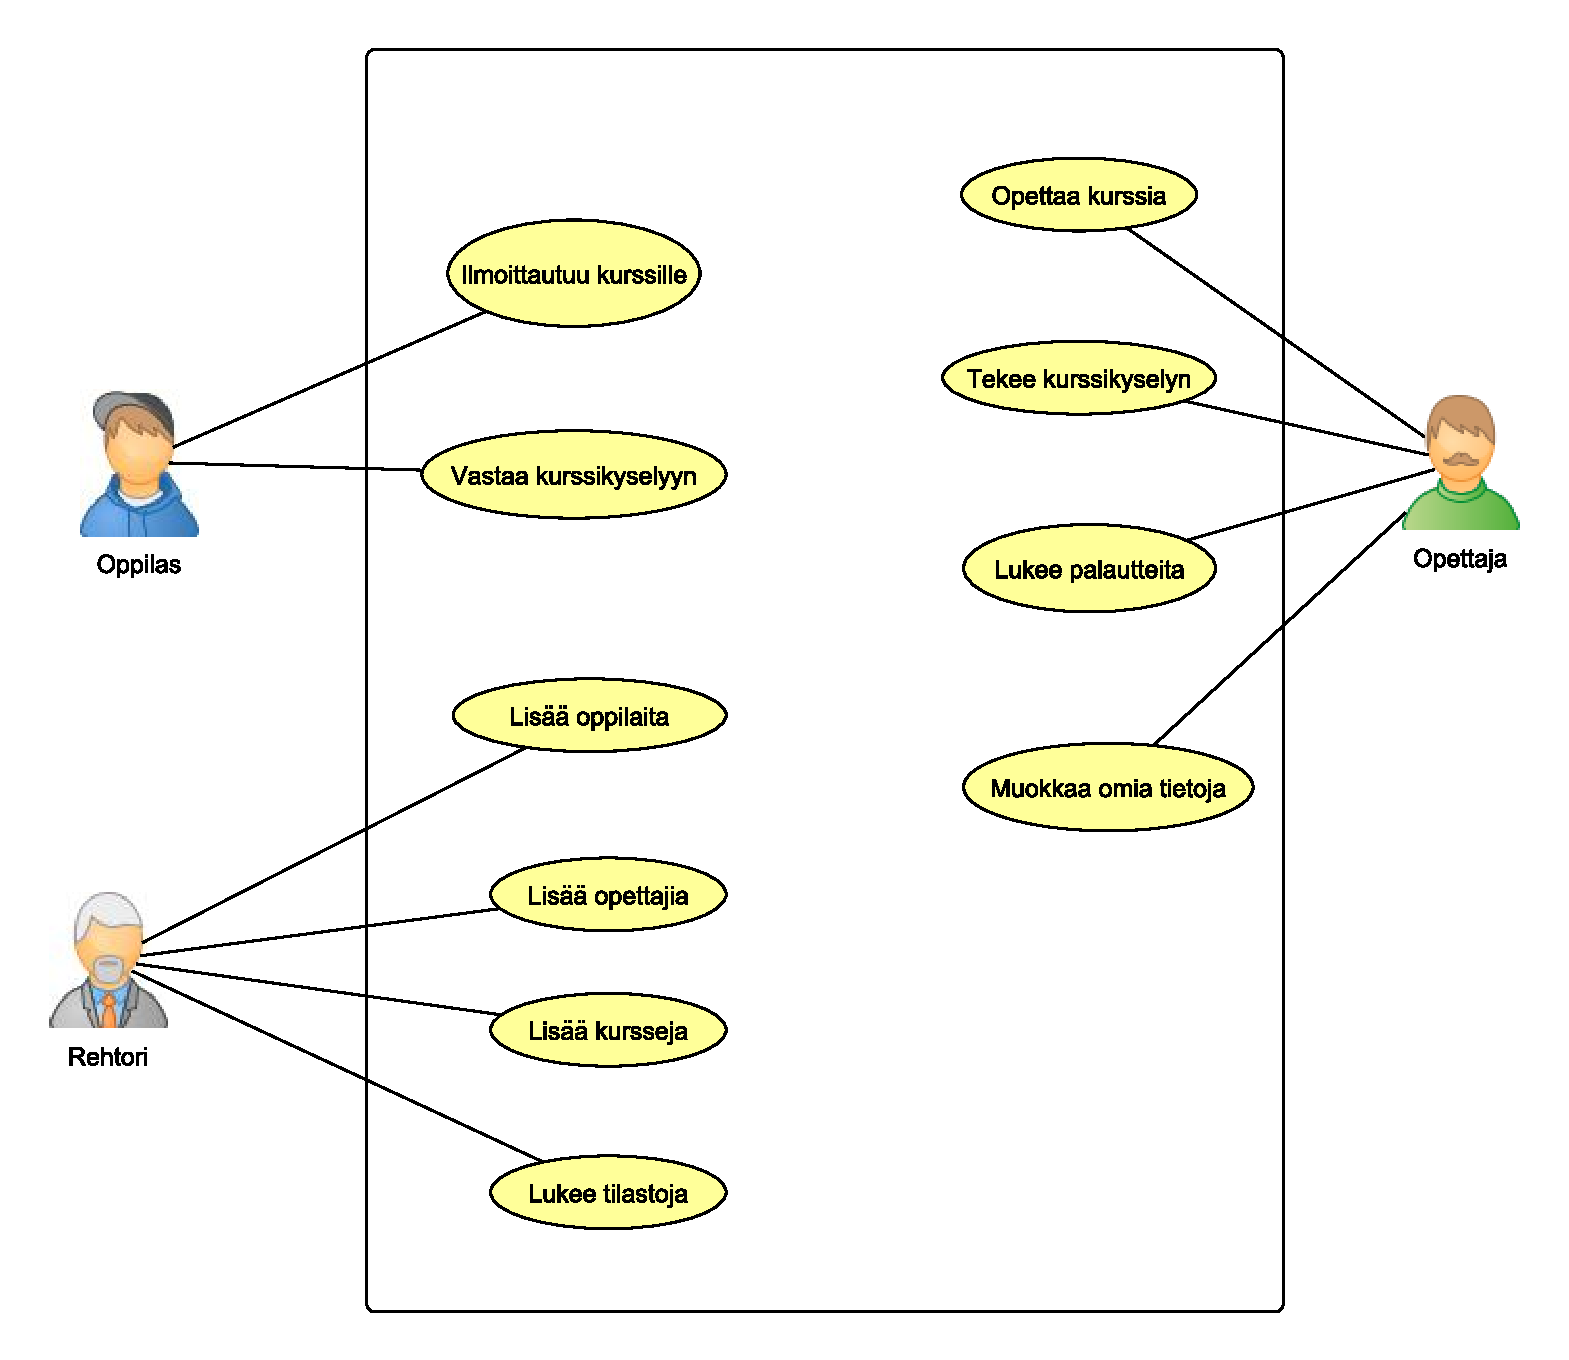
\includegraphics[width=0.95\textwidth]{kayttotapauskaavio.eps}
  \caption{Käyttötapauskaavio.}
\end{figure}

\subsection{Käyttäjäryhmät}

\begin{description}
  \item[Oppilas] Oppilas opiskelee oppilaitoksessa. Suorittaa kursseja 
  suunnitelmansa mukaisesti.
  \item[Opettaja] Opettaa oppilaitoksessa. Pitää kursseja opetusvelvollisuuden
  mukaisesti.
  \item[Rehtori] Johtaa oppilaitosta ja valvoo, että kaikki toimii suunnitelmien
  mukaisesti.
\end{description}

\subsection{Käyttötapauskuvaukset}

\subsubsection*{Oppilaan käyttötapaukset}

Kurssikyselyyn vastaaminen:

Käy vastaamasssa kurssille tehtyyn kurssikyselyyn. Kurssikyselyjen etusivulla on
listattuna kaikki kurssit, joille on tehty kurssikysely ja kysely on aktiivisena.
Oppilas klikkaa kurssia ja antaa oppilasnumeronsa, jolla varmistetaan, että kyselyyn
vastaa kurssilla olevat oppilaat. Oppilas voi käydä muuttamassa vastauksiaan niin
kauan kuin kysely on aktiivinen ja se tapahtuu samalla tavalla kuin ensimmäisellä
kerralla kurssikyselyyn vastaaminen. Oppilas näkee tällöin aikaisemmat vastaukset
ja voi muuttaa niitä.

\subsubsection*{Opettajan käyttötapaukset}

Kurssikyselyjen tekeminen:

Opettaja kirjautuu omilla tunnuksillaan kurssikyselyjen etusivulta.
Opettaja näkee kurssit, joita hän opettaa ja nappia painamalla voi lisätä kurssille
kyselyn tai muokata jo aikaisemmin tehtyä kyselyä. Kyselyjen muokkaussivulla
kysymys lisätään valitsemalla valmiiksi tietokantaan talletettuja kysymyksiä ja
määrittelemällä onko se monivalinta kysymys vai haluaako opettaja oppilaan kirjoittavan
ominsanoin tekstikenttään vastauksen.

Palautteiden lukeminen:

Opettaja voi lukea oppilaiden kurssikyselyyn antamia vastauksia. Hän voi lukea
yksittäisen oppilaan vastaukset ja samalla näkee saman kurssin monivalintakysymyksien
vastauksien mediaanit.

\subsubsection*{Rehtorin käyttötapaukset}

Tietokantojen hallinnointi:

Lisää opettajia, oppilaita ja kursseja tietokantaan, sekä lisää opiskelijat
ilmoittautumisien mukaan kursseille. Näkee kurssien kyselyihin vastanneiden
määrän ja kurssilla olevien oppilaiden määrän.

\section{Järjestelmän tietosisältö}

\begin{figure}[!h]
  \centering
  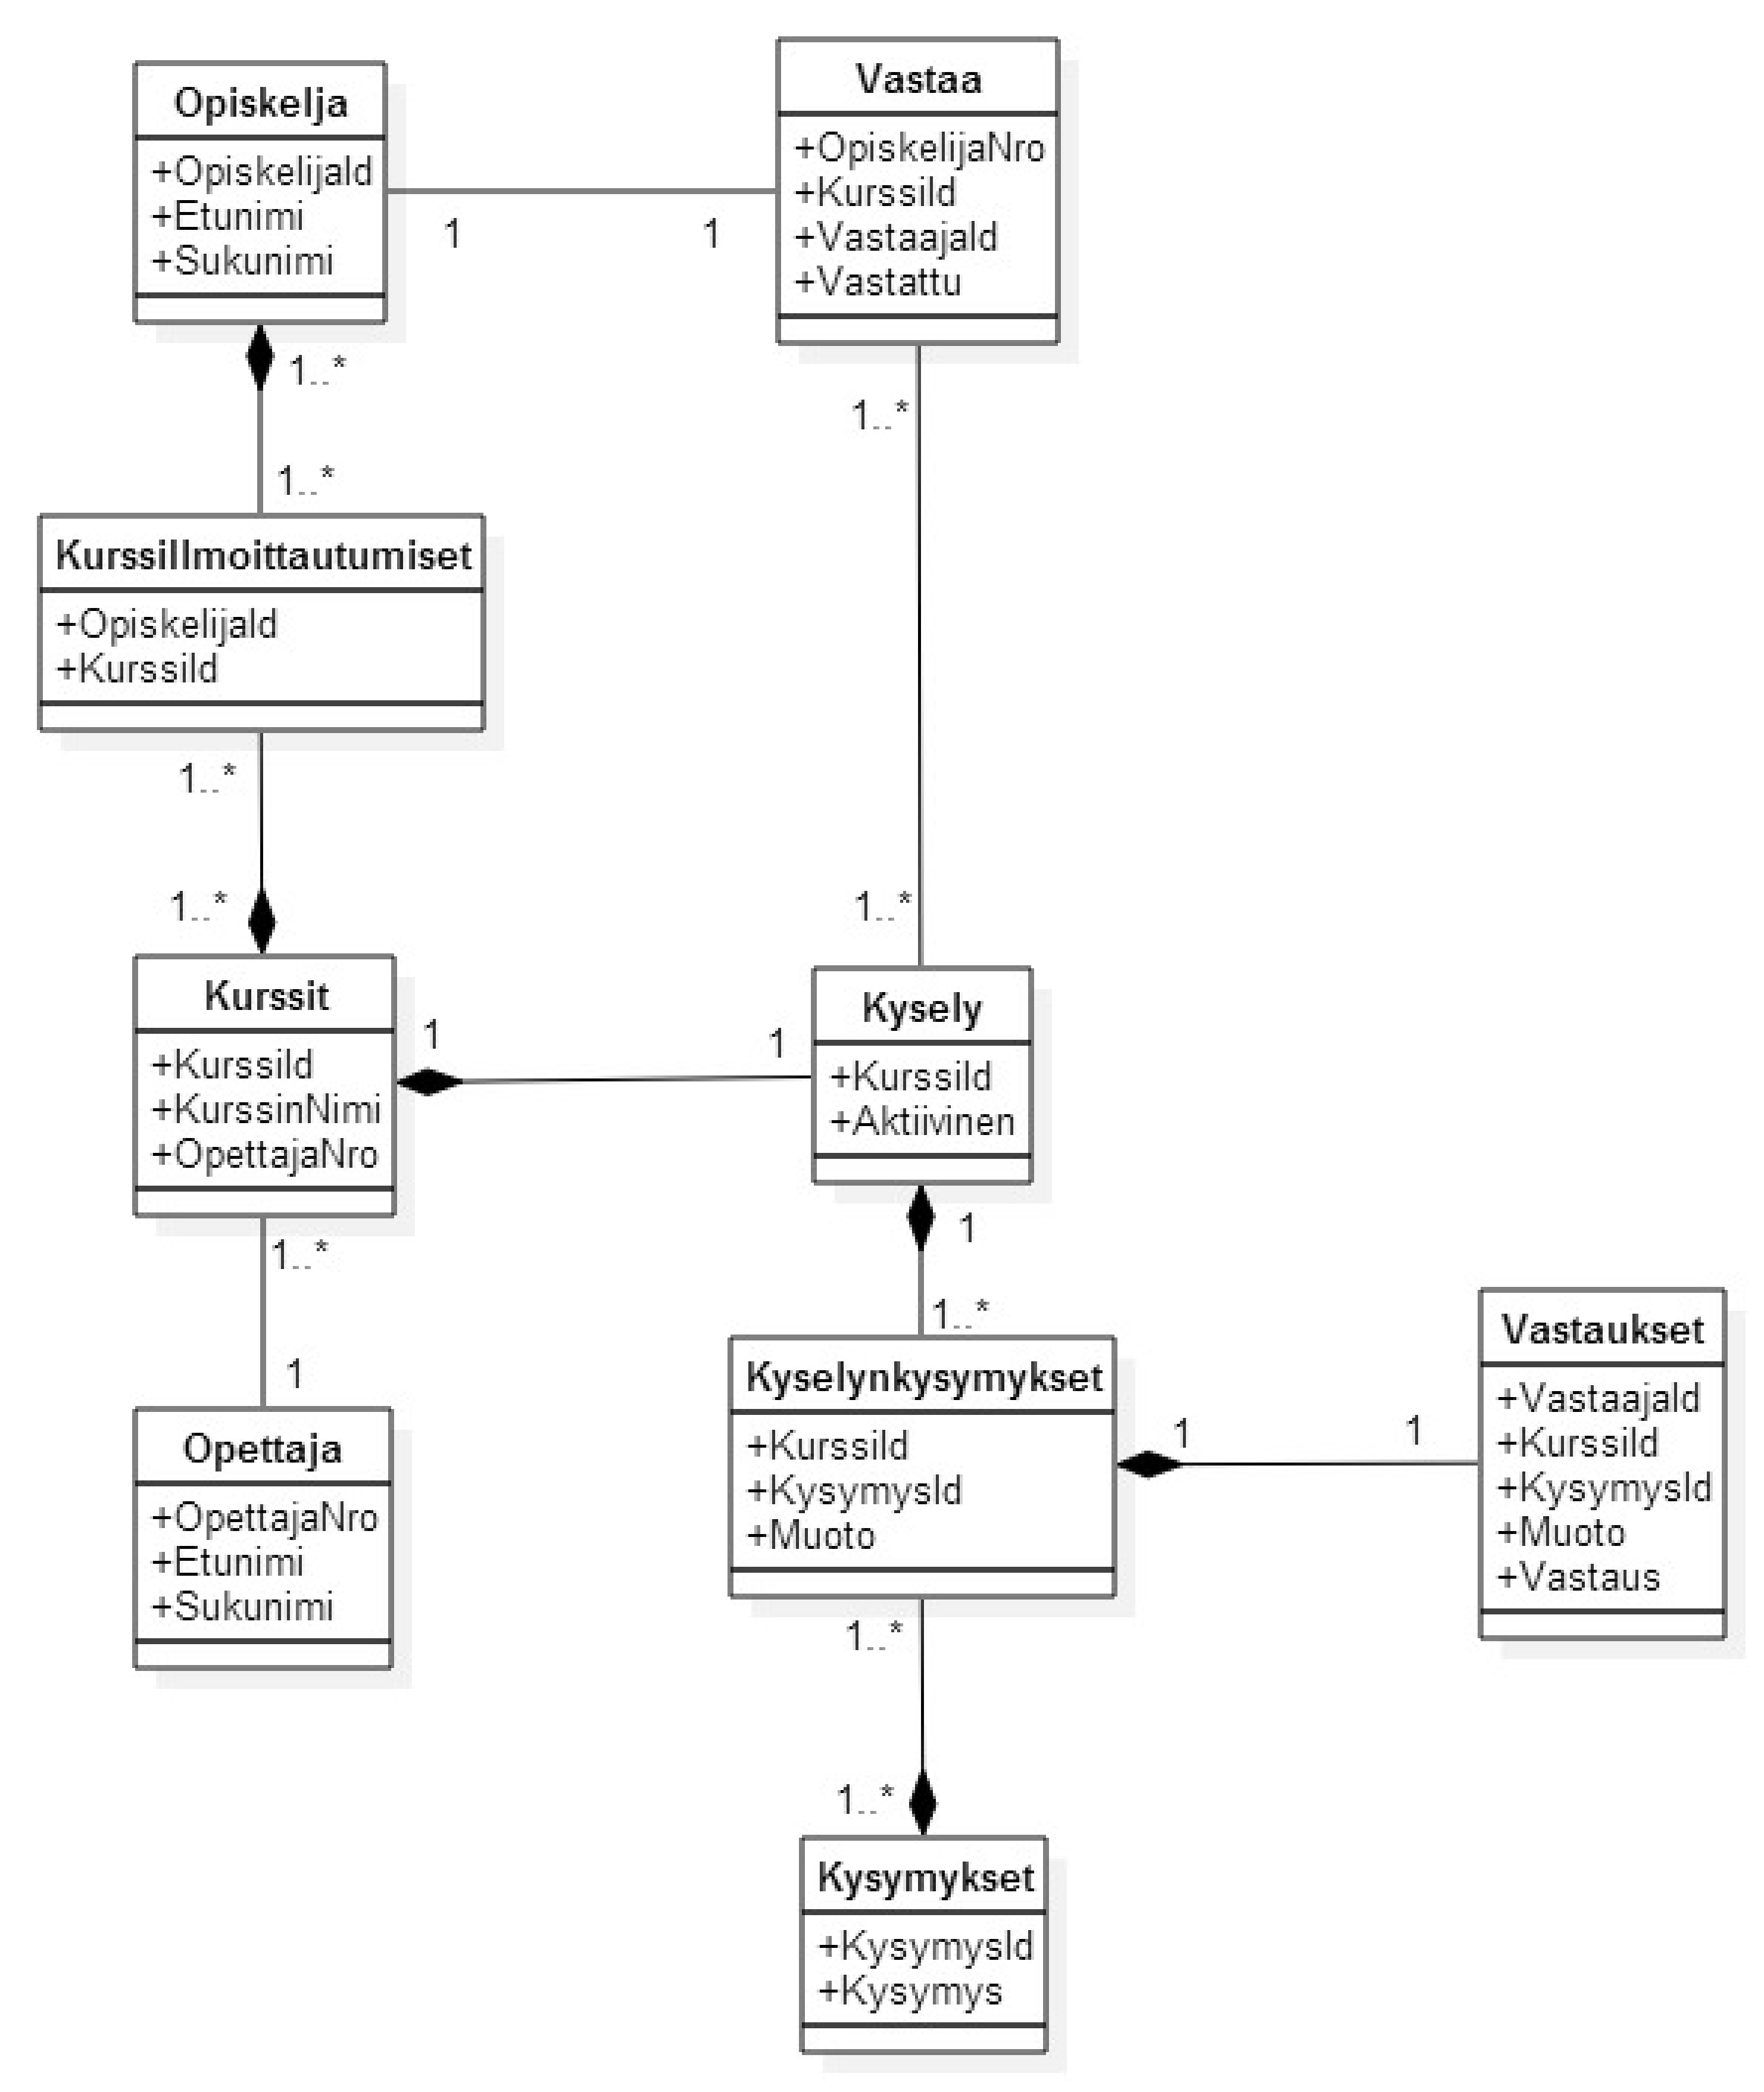
\includegraphics[width=0.7\textwidth]{kasitekaavio.eps}\\
  \caption{Käsitekaavio}
\end{figure}


\subsubsection*{Kysymykset}

\begin{table}[!h]
\begin{tabular}{|c|p{5cm}|p{5cm}|}
  \hline
  % after \\: \hline or \cline{col1-col2} \cline{col3-col4} ...
  \textbf{Attribuutti} & \textbf{Arvojoukko} & \textbf{Kuvailu} \\
  \hline
  KysymysId & Kokonaisluku & Kysymyksen tunnus, joilla kysymykset voidaan
  erottaa \\
  \hline
  kysymys & Merkkijono, max. 150 merkkiä & Kysymys, joka voidaan liittää
  liittää kyselyyn \\
  \hline
\end{tabular}
\end{table}

\subsubsection*{Opettaja}

\begin{table}[!h]
\begin{tabular}{|c|p{5cm}|p{5cm}|}
  \hline
  % after \\: \hline or \cline{col1-col2} \cline{col3-col4} ...
  \textbf{Attribuutti} & \textbf{Arvojoukko} & \textbf{Kuvailu} \\
  \hline
  OpettajaNro & Kokonaisluku & Identifioi opettajan \\
  \hline
  Etunimi & Merkkijono, max. 20 merkkiä & Opettajan etunimi \\
  \hline
  Sukunimi & Merkkijono, max. 30 merkkiä & Opettajan sukunimi \\
  \hline
\end{tabular}
\end{table}

\subsubsection*{Opiskelija}

\begin{table}[!h]
\begin{tabular}{|c|p{5cm}|p{5cm}|}
  \hline
  % after \\: \hline or \cline{col1-col2} \cline{col3-col4} ...
  \textbf{Attribuutti} & \textbf{Arvojoukko} & \textbf{Kuvailu} \\
  \hline
  OpiskelijaNro & Kokonaisluku & Identifioi opiskelijan \\
  \hline
  Etunimi & Merkkijono, max. 20 merkkiä & Opiskelijan etunimi \\
  \hline
  Sukunimi & Merkkijono, max. 30 merkkiä & Opiskelijan sukunimi \\
  \hline
\end{tabular}
\end{table}

\subsubsection*{Kurssit}

\begin{tabular}{|c|p{5cm}|p{5cm}|}
  \hline
  % after \\: \hline or \cline{col1-col2} \cline{col3-col4} ...
  \textbf{Attribuutti} & \textbf{Arvojoukko} & \textbf{Kuvailu} \\
  \hline
  KurssiId & Kokonaisluku & Identifioi kurssin \\
  \hline
  OpettajaNro & Kokonaisluku & Kurssin opettajan opettajanumero \\
  \hline
  KurssinNimi & Merkkijono, max. 40 merkkiä & Kurssin nimi \\
  \hline
\end{tabular}

\subsubsection*{Kurssi-ilmoittautumiset}

\begin{tabular}{|c|c|p{5cm}|}
  \hline
  % after \\: \hline or \cline{col1-col2} \cline{col3-col4} ...
  \textbf{Attribuutti} & \textbf{Arvojoukko} & \textbf{Kuvailu} \\
  \hline
  KurssiId & Kokonaisluku & Kertoo mikä kurssi on kyseessä \\
  \hline
  OpiskeliNro & Kokonaisluku & Kertoo, kuka opiskelija on ilmoittautunut
  kurssille \\
  \hline
\end{tabular}

\subsubsection*{Kysely}

\begin{table}[!h]
\begin{tabular}{|c|c|p{5cm}|}
  \hline
  % after \\: \hline or \cline{col1-col2} \cline{col3-col4} ...
  \textbf{Attribuutti} & \textbf{Arvojoukko} & \textbf{Kuvailu} \\
  \hline
  KurssiId & Kokonaisluku & Kertoo, minkä kursssin kurssikysely on \\
  \hline
  Aktiivinen & Merkkijono, max. 5 merkkiä & Kertoo, onko kysely käynnissä vai ei \\
  \hline
\end{tabular}
\end{table}

\clearpage
\section{Relaatiotietokantakaavio}

\begin{figure}[!h]
  \centering
  % Requires \usepackage{graphicx}
  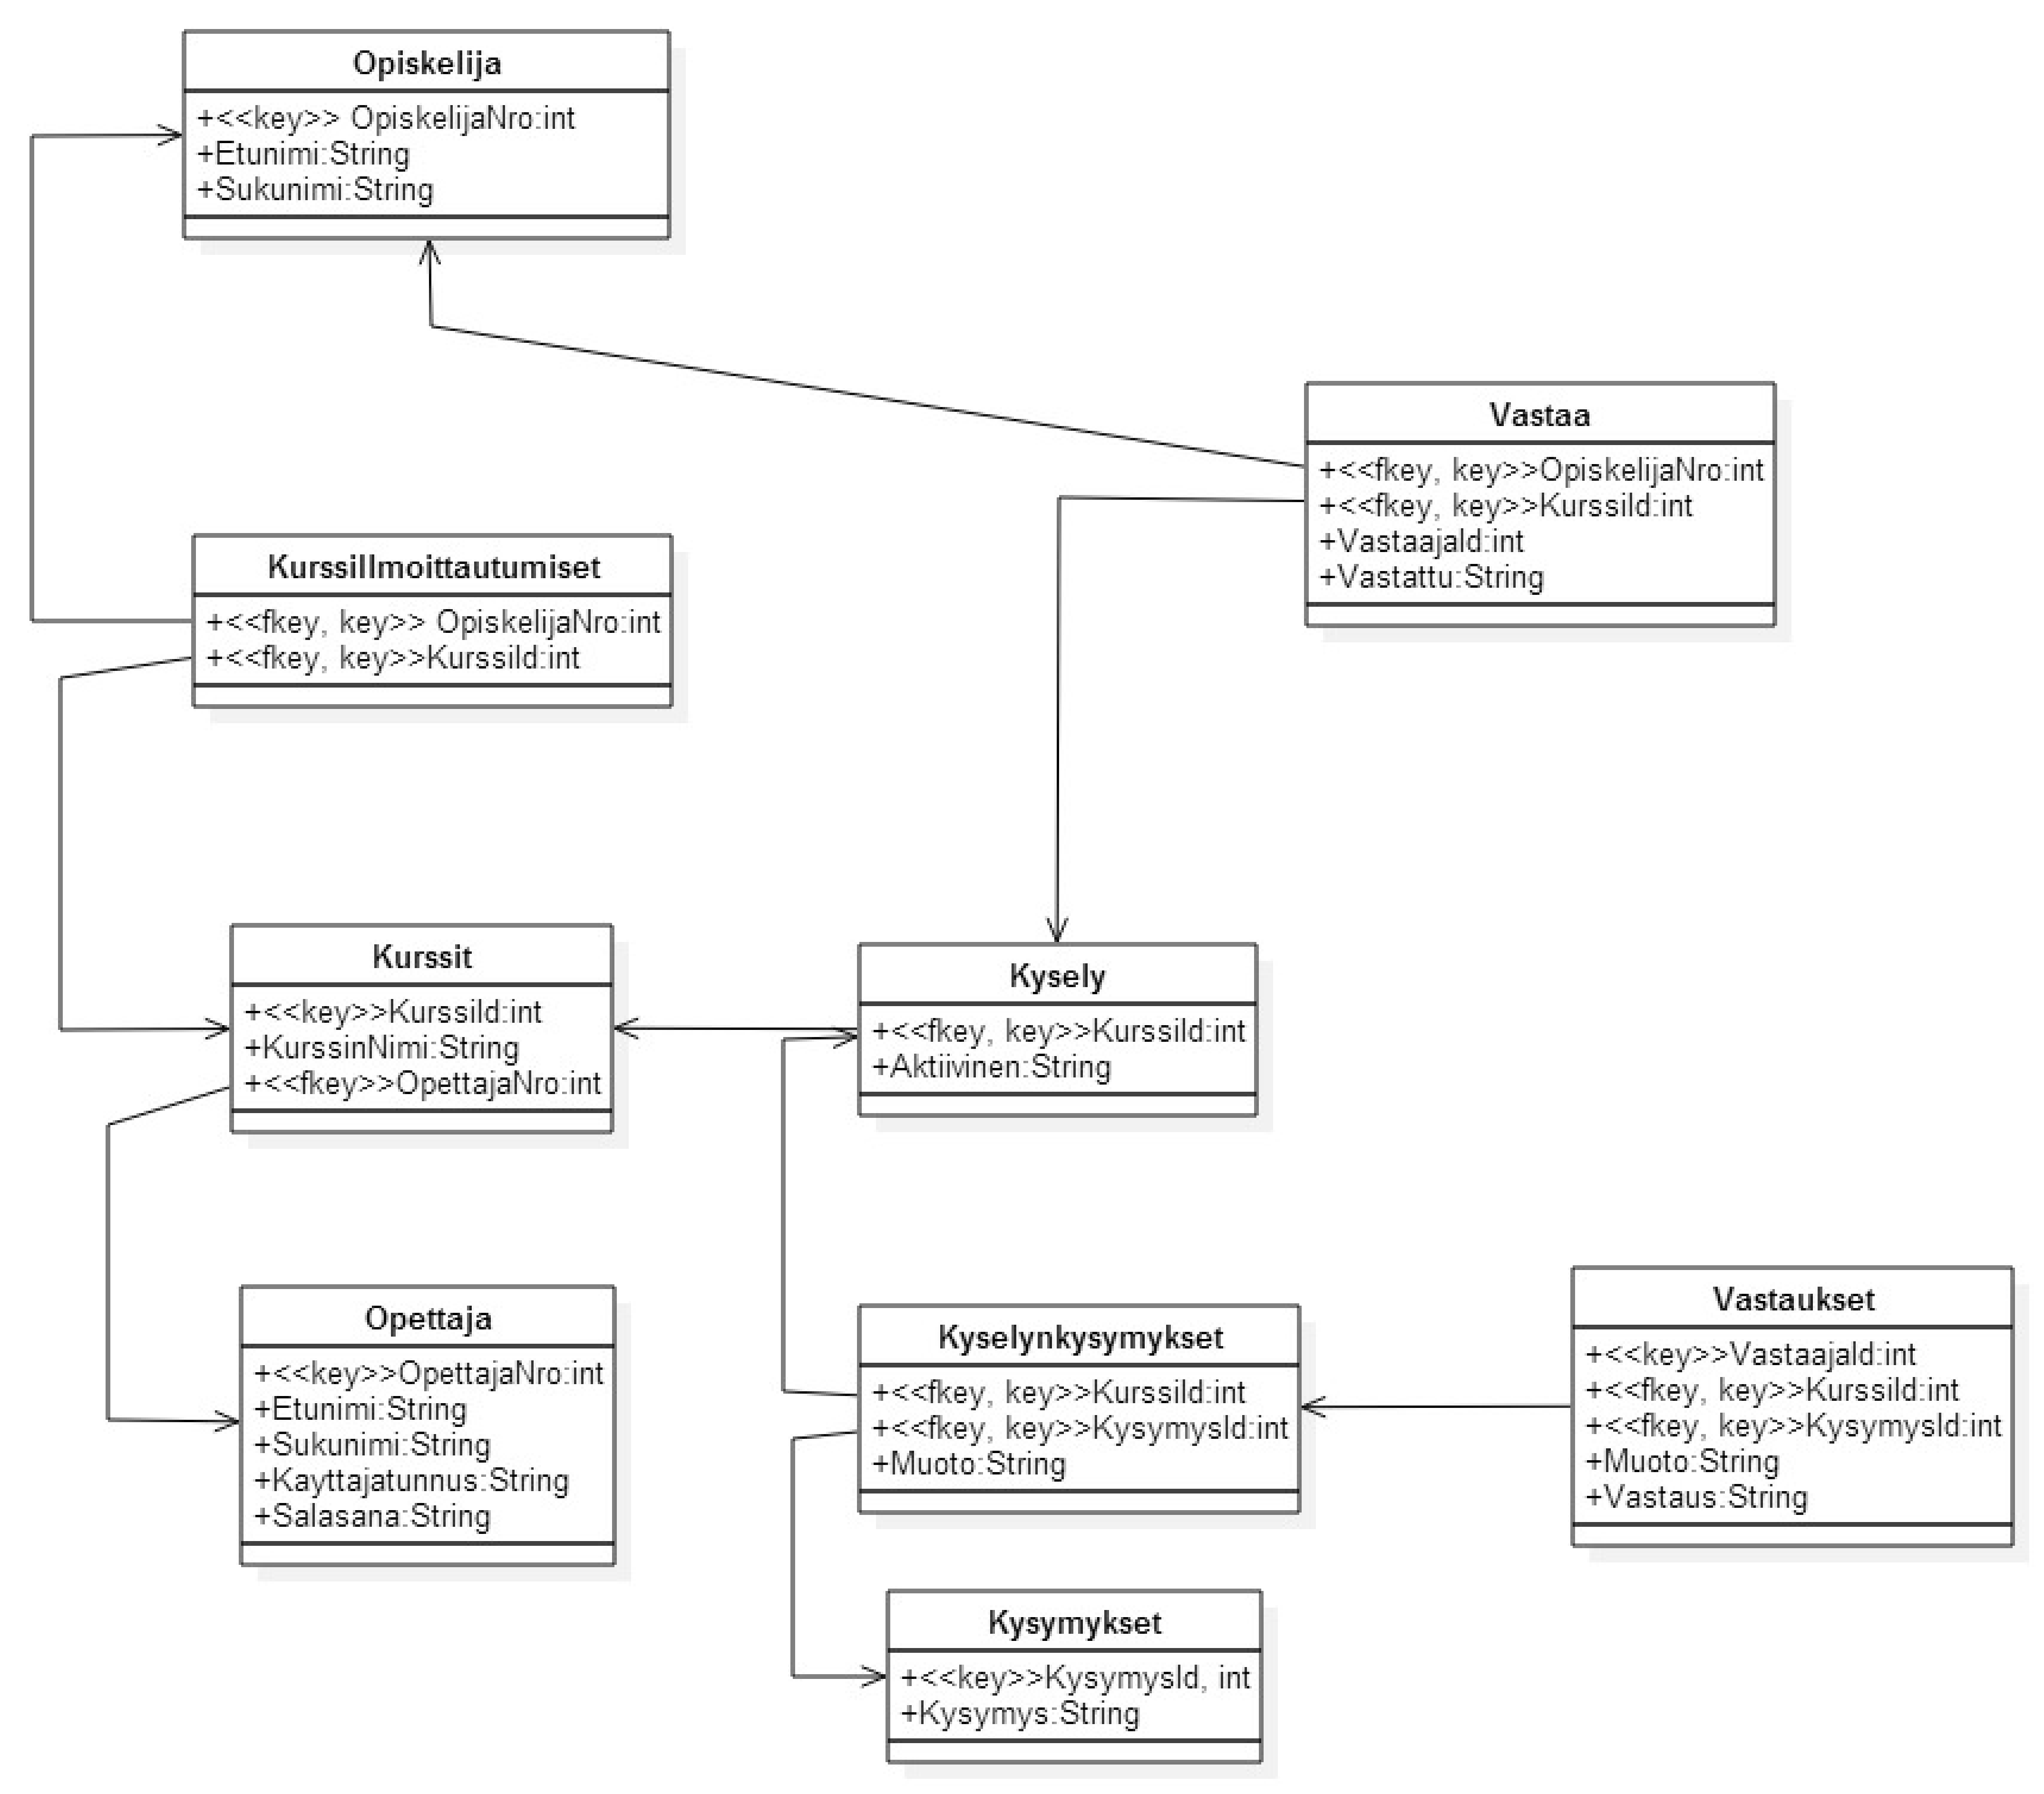
\includegraphics[width=\textwidth]{relaatiotietokantakaavio.eps}\\
  \caption{Relaatiotietokantakaavio.}
\end{figure}


\section{Järjestelmän yleisrakenne}

Sovellusta tehdessä on noudatettu MVC-mallia. Kontrollerit sijaitsevat 
hakemistojen juuressa, näkymät \verb'views'-kansiossa ja mallit 
\verb'libs/models'-kansiossa. Apufunktiot ovat \verb'libs'-kansiossa. Malliluokissa 
tapahtuu tietokantaoperaatiot, kyselyt, tallentaminen ja tietojen päivittäminen.
Tietokantataulujen luonti tiedosto on sijoitettu \verb'sql'-kansioon.

\clearpage
\section{Käyttöliittymä ja järjestelmän komponentit}

\begin{figure}[!h]
  \centering
  % Requires \usepackage{graphicx}
  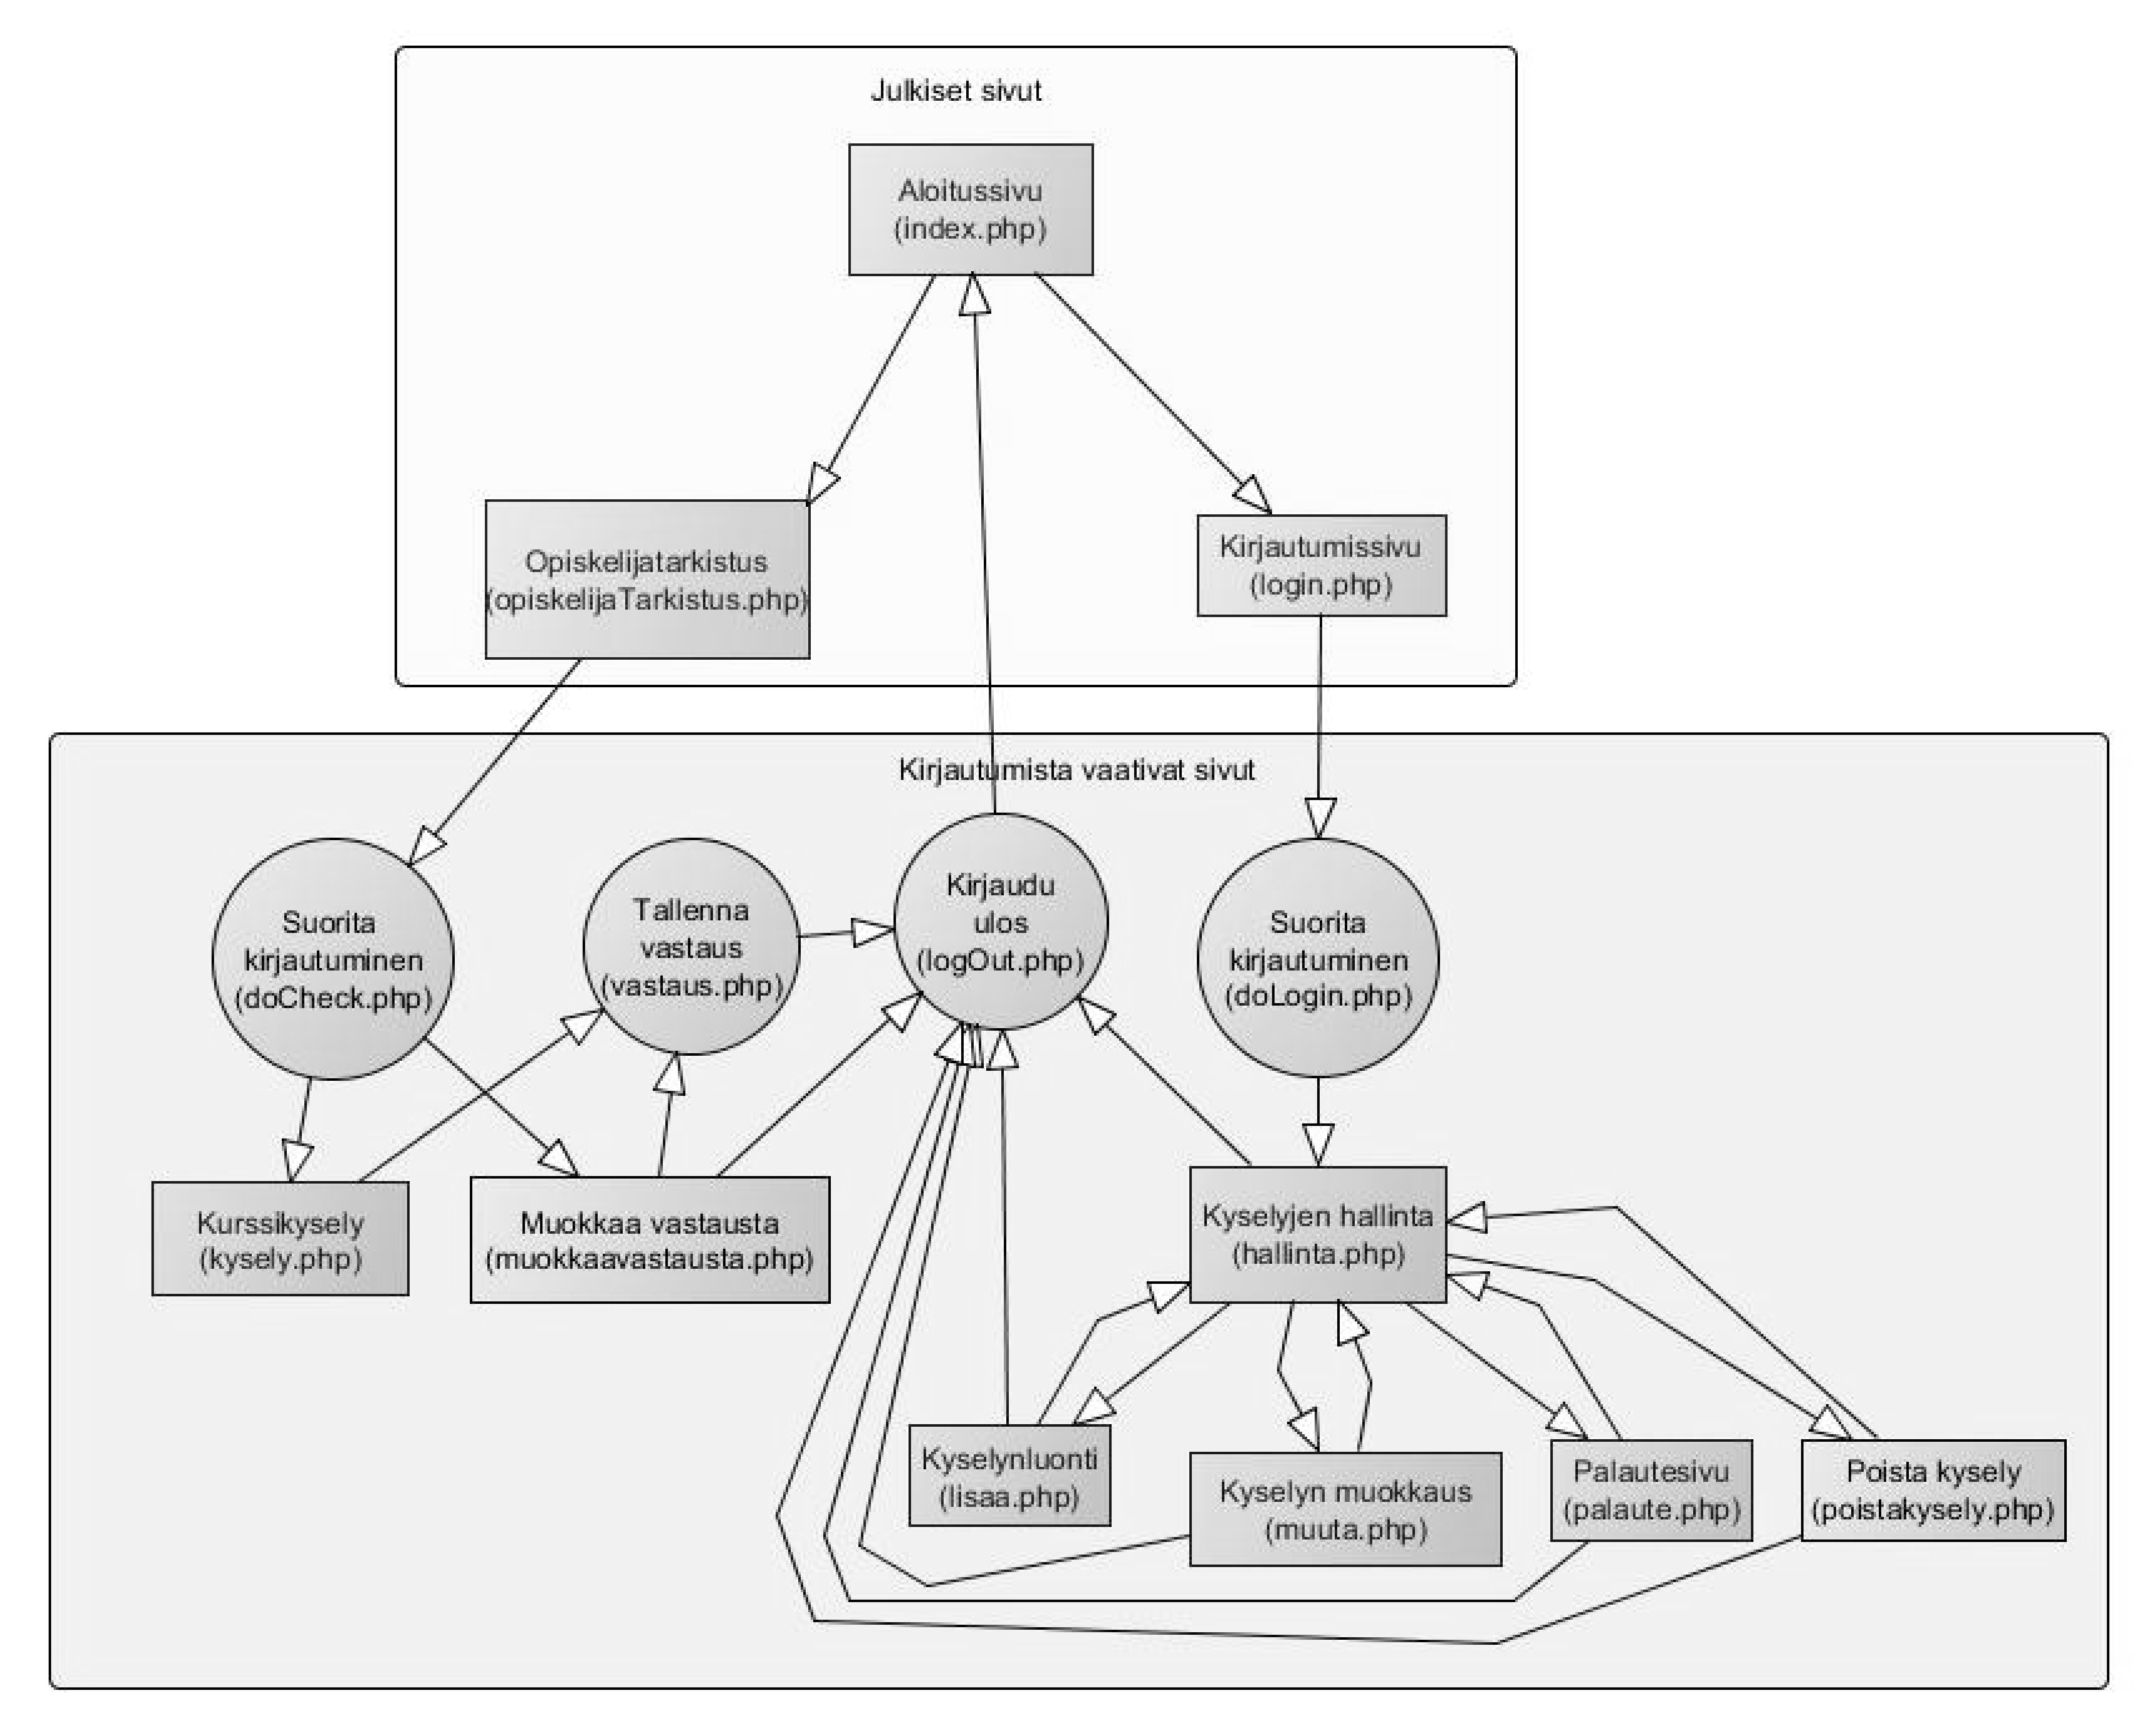
\includegraphics[width=0.95\textwidth]{kayttoliittyma.eps}\\
  \caption{Käyttöliittymä}
\end{figure}


\section{Asennustiedostot}

Sovellus on asennettu users-palvelimelle kansioon \verb'htdocs/TiSoHa'. Kansiossa
on kontrollerit ja näkymät sijaitsevat kansiossa \verb'htdocs/TiSoHa/views'. Malliluokat
sijaitsevat \verb'htdocs/TiSoHa/libs/models'-kansiossa ja kansiossa \verb'libs' on
apufunktioita. Kansiossa \verb'htdocs/TiSoHa/sql' sijaitsee tietokantataulujen 
luonti- ja poisto-tiedostot, sekä testidatan lisäys tiedosto.

Asenna sovellus kopioimalla sen tiedostot palvelimen nettiin näkyvään hakemistoon 
(esim. usersin htdocs-hakemisto) ja \verb'views'-, \verb'libs'-, \verb'libs/models'- 
sisällöt samannimisiin kansioihin. 

\section{Käynnistysohje}

Harjoitustyö sijaitsee osoitteessa\\ \verb"http://tpheiska.users.cs.helsinki.fi/TiSoHa/index.php".
Opettajana voi kirjautu sisään tunnuksilla: \verb'opettaja' ja salasanana \verb'salasana'
tai \verb'ope' ja salasanana \verb'salasana'. Kyselyyn voi mennä vastaamaan
oppilasnumeroilla \verb'1' ja \verb'2'.

\section{Testaus}

Olen testannut ohjelmaa kokeilemalla eri toimintoja, kuten kyselyn lisäämistä,
poistoa, aktivointia, sulkemista, opiskelijana kyselyyn vastaamista, uudelleen
vastaamista ja url:n perusteella uudelleen kyselysivulle menemistä. Lisäsin
toisen opettaja ja varmistuin, että kirjautuneena opettaja saa vain omat kurssit
näkyviin ja voi tehdä kyselyjä vain omille kursseille. Varmistuin myös, että
opettaja näkee vain omiin kursseihin ja niihin liittyviin kyselyihin liittyvät
vastaukset. Kokeilin opiskelijana vastatessa sijoittaa html:ää väliin ja se ei
tuottanut ongelmia.

Ohjelmasta puuttuu vielä käyttäjä, joka voi lisätä opettajia, oppilaita ja kursseja.
Tämä käyttäjä ei voi lukea kyselyiden vastauksia, mutta hänen tulisi saada tieto
kyselyihin vastanneiden ja kurssilla olijoiden määristä. Kyselyitä tehdessä kysymykset
voi valita vain tietokantaan talletetuista kysymyksistä, mutta tarkoitus on vielä
muuttaa järjestelmää niin, että jos tietokannassa ei löydy mieleistä kysymystä, niin
sen voi itse kirjoittaa ja samalla se talletetaan tietokantaan. Tällöi pitää myös
varmistua, että sitä ei todella ole jo talletettuna tietokantaan.

\section{Omat kokemukset}

Sovelluksen teossa helpointa oli tietokantataulujen suunnittelu ja luonti. Vaikeuksia
alkoi jo tulla heti tietokantakyselyjen tekemisessä johtuen kauan sitten suoritetusta
tietokantojen perusteet kurssista ja siitä, että käytännössä kurssin jälkeen ei
tullut tarvetta käyttää tai muistella SQL:ää. PHP:llä en ollut koskaan tehnyt mitään
ja oli mukava huomata, miten sitä voi kirjoitta html:n sekaan ja helpottaa sivujen
tekoa. Aikataulu oli todella tiukka, enkä mitenkään meinannut pysy niissä. Työssä
tuli kokoajan niin paljon uutta, että piti käyttää paljon aikaa niiden
opetteluun. Kirjoitusvirheet koodissa tuottivat paljon työtä ja veivät 
erittäin paljon aikaa, että ne löysi ja sai kaiken toimimaan niin kuin oli ajatellut.


\end{document}
